%\VignetteIndexEntry{Using PING with paired-end sequencing data}
%\VignetteDepends{PING,parallel}
%\VignetteKeywords{Preprocessing, ChIP-Seq, Sequencing}
%\VignettePackage{PING}
\documentclass[11pt]{article}
\usepackage{Sweave}
\usepackage{underscore}
%\usepackage{hyperref}
%\usepackage{url}
%\usepackage{color, pdfcolmk}
%\usepackage[authoryear,round]{natbib}
%\bibliographystyle{plainnat}
%\usepackage[hmargin=2cm, vmargin=3cm]{geometry}
 %Introduce newlines automatically in R code


%\newcommand{\scscst}{\scriptscriptstyle}
%\newcommand{\scst}{\scriptstyle}

\title{Using PING with Paired-End sequencing data}
\author{Xuekui Zhang\footnote{ubcxzhang@gmail.com}, Sangsoon
Woo\footnote{swoo@fhcrc.org}, Raphael Gottardo\footnote{rgottard@fhcrc.org} and
Renan Sauteraud\footnote{rsautera@fhcrc.org}}

\begin{document}
%To display nice multilines chunks of code

\maketitle



\textnormal {\normalfont}
This vignette presents a workflow to use PING on paired-end sequencing data.

\tableofcontents
%%%%%%%%%%%%%%%%%%%%%%%%%%%%%%%%%%%%%%%%%%%%%%%%%%%%%%%%%%%%%%%%%%%%%%%%%%%%%%%
\newpage


\section{Licensing and citing}

Under the Artistic License 2.0, you are free to use and redistribute this software. 

If you use this package for a publication, we would ask you to cite the following: 

\begin{itemize}
\item[] Xuekui Zhang, Gordon Robertson, Sangsoon Woo, Brad G. Hoffman, and Raphael Gottardo. (2012). Probabilistic Inference for Nucleosome Positioning with MNase-based or Sonicated Short-read Data. PLoS ONE 7(2): e32095.
\end{itemize}


\section{Introduction}
For an introduction to the biological background and PING method, please refer to the PING user guide.


\section{PING analysis steps}
A typical PING analysis consists of the following steps:
\begin{enumerate}
  \item Extract reads and chromosomes from bam files.
  \item Segment the genome into candidate regions that have sufficient aligned reads via `segmentPING'
  \item Estimate nucleosome positions and other parameters with PING
  \item Post-process PING predictions to correct certain predictions
\end{enumerate}

As with any R package, you should first load it with the following command:

\begin{Schunk}
\begin{Sinput}
> library(PING)
\end{Sinput}
\end{Schunk}

\section{Data Input and Formatting}
As with the Single-End \texttt{PING}, the input used for the segmentation step is a \texttt{GRanges} object.

Because Paired-End sequencing data often comes in the form of a .bam file, we provide a function to convert these files into \texttt{GRanges} with all the appropriate information.
We provide a small bam file with two chromosomes of the yeast to be used as an example in this vignette.

\begin{Schunk}
\begin{Sinput}
> yeastBam <- system.file("extdata/yeastChrI_M.bam", package = "PING")
\end{Sinput}
\end{Schunk}

\begin{Schunk}
\begin{Sinput}
> gr <- bam2gr(bamFile = yeastBam)
\end{Sinput}
\begin{Soutput}
Chromosome  chrI 
Chromosome  chrM 
\end{Soutput}
\end{Schunk}
$gr$ is a \texttt{GRanges} object containing all the reads from the .bam file. 


\section{PING analysis}

\subsection{Genome segmentation}
PING is used the same way for paired-end and single-end sequencing data. The
function \texttt{segmentPING} will decide which segmentation method should be
used based on the arguments provided. 
When dealing with paired-end data, four new arguments have to be passed to the
function: a chromosome chr and three parameters used in candidate region
selection: islandDepth, min_cut and max_cut.

These arguments control the size and required coverage for a region to be
considered as a candidate.

In order to improve the computational efficiency of the PING package, if you
have access to multiple cores we recommend that you do parallel computations via
the \texttt{parallel} package. In what follows, we assume that \texttt{parallel}
is installed on your machine. If it is not, you could omit the first line, and
calculations will occur on a single CPU. By default the command is not run. Note
that the \texttt{segmentPING} and \texttt{PING} functions will automatically
detect whether you have initialized a cluster and will use it if you have.

\begin{Schunk}
\begin{Sinput}
> library(parallel)
\end{Sinput}
\end{Schunk}


\begin{Schunk}
\begin{Sinput}
> segPE <- segmentPING(gr, chr = "chrM", islandDepth = 3, min_cut = 50, 
     max_cut = 1000)
\end{Sinput}
\end{Schunk}

It returns a \texttt{segReadsListPE} object.


\subsection{Parameter estimation}
The only difference when using \texttt{PING} for paired-end data is the argument PE that has to be set to TRUE.

%paraP<-setParaPriorPING(xi=150, rho=1.2, alpha=12, beta=20000, lambda=-0.000064, dMu=200)
\begin{Schunk}
\begin{Sinput}
> ping <- PING(segPE, PE = TRUE)
\end{Sinput}
\end{Schunk}
The returned object is of class pingList and can be post-processed.


\section{Post-processing PING results}
Here again, we set the argument PE to TRUE, and use postPING normally.

\begin{Schunk}
\begin{Sinput}
> {
     sigmaB2 = 3600
     rho2 = 15
     alpha2 = 98
     beta2 = 2e+05
 }
> PS = postPING(ping, segPE, rho2 = rho2, alpha2 = alpha2, beta2 = beta2, 
     sigmaB2 = sigmaB2, PE = TRUE)
\end{Sinput}
\begin{Soutput}
 The 5 Regions with following IDs are reprocessed for singularity problem: 
(0.783,110]84   (110,218]37   (110,218]50   (110,218]76   (110,218]79 
           84           146           159           185           188 

 The 1 Regions with following IDs are reprocessed for atypical delta: 
[1] 149
[1] "No predictions with atypical sigma"

 The 138 regions with following IDs are reprocessed for Boundary problems: 
[1]  4 17 25 38 40 47
\end{Soutput}
\end{Schunk}
The result output $PS$ is a dataframe that contains estimated parameters of each nucleosome, users can use write.table command to export the selected columns of the result.
\begin{Schunk}
\begin{Sinput}
> head(PS, 3)
\end{Sinput}
\begin{Soutput}
     ID  chr         w       mu    delta  sigmaSqF sigmaSqR        se     score
88   28 chrM 0.3926403 11626.37 119.9353 1015.1863 941.0201 11.636744 0.4903682
367 117 chrM 0.2141183 47288.11 129.3172  803.2646 808.8207  7.837640 0.4402827
490 157 chrM 0.6212985 63073.44 131.2461  960.0974 879.2203  5.211408 0.4397749
       scoreF    scoreR minRange maxRange       seF       seR rank
88  0.5021658 0.4781146    11409    12499 12.847227 11.572460    1
367 0.3881176 0.4922684    46653    47604  9.068648  8.931158    2
490 0.4303097 0.4496658    62728    63760  5.678614  6.750760    3
\end{Soutput}
\end{Schunk}

\section{Analyzing the prediction}
\texttt{PING} comes with a set of tools to export or visualize the prediction.
Here, we only show how to export the results into bed format for further use
and how to make a quick plot to summarize the prediction. For more information
on how to export the results or make more complex plots, refer to the section
`Result output' of PING vignette.

The function \texttt{makeRangedDataOutput} offers a simple way to convert the
prediction results into a \texttt{RangedData} object ready to be exported with
the package \texttt{rtracklayer}.

\begin{Schunk}
\begin{Sinput}
> rdBed <- makeRangedDataOutput(PS, type = "bed")
> library(rtracklayer)
> export(rdBed, "nucPrediction.bed")
\end{Sinput}
\end{Schunk}

The exported file contain all the predicted nucleosomes displayed in bed format
and ranked by score.

\vspace{10pt}
For PE data, the function \texttt{plotSummary} will generate a plot displaying 
the coverage by the reads used as input and the predicted position of the
nucleosomes of $PS$ for the given ranges as well as theur associated prediction score.

\begin{Schunk}
\begin{Sinput}
> plotSummary(PS, gr, chr = "chrM", from = 1000, to = 4000, PE = TRUE)
\end{Sinput}
\end{Schunk}
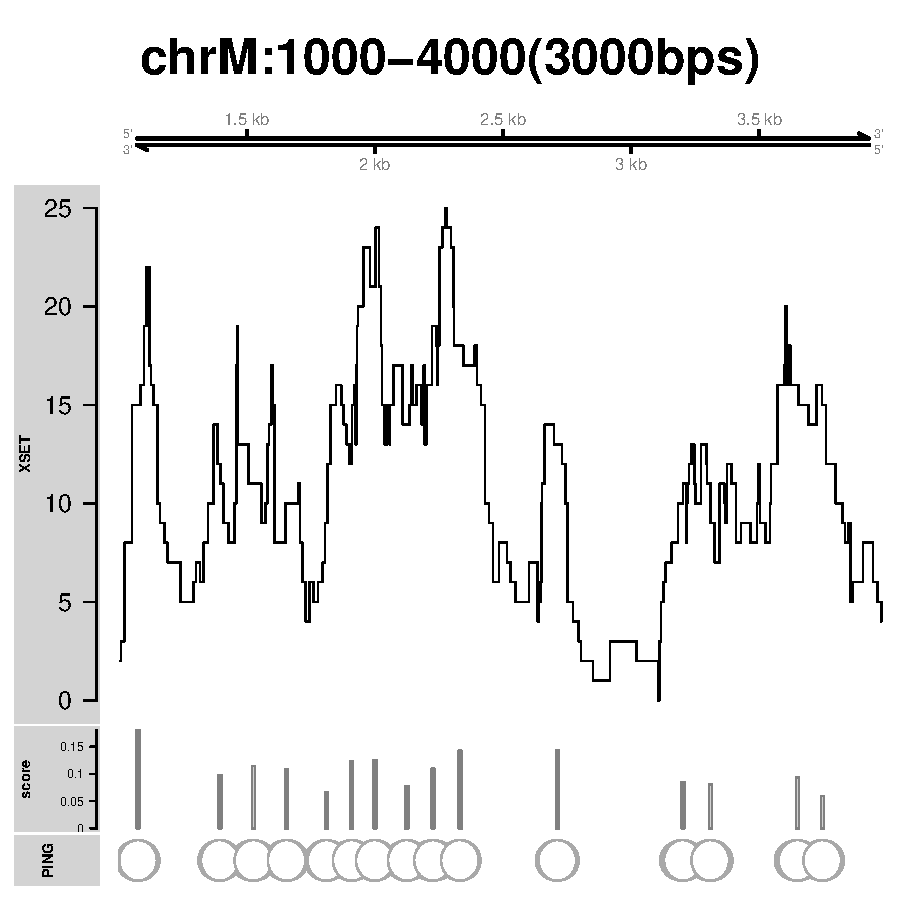
\includegraphics{PING-PE-plotSummary-PE}

Note that the argument PE should be set to TRUE. All the arguments for this function will work for Paired-end data as well. Refer to PING vignette and ?plotSummary for more information.

\end{document}
